\documentclass[12pt]{beamer}
\usepackage{cmap}
\usepackage[T2A]{fontenc}
\usepackage[utf8]{inputenc}
\usepackage{ifluatex}
\usefonttheme[onlymath]{serif}
\usepackage{svg}
\usepackage{enumerate}
\usepackage{hyperref}
\usepackage{mathtools}
\setbeamertemplate{footline}[frame number]
\definecolor{beamer@darkgreen}{rgb}{0,0.6,0}
\setbeamercolor{normal text}{fg=black,bg=white}
\setbeamercolor{title}{fg=black,bg=beamer@darkgreen}
\setbeamercolor{frametitle}{fg=black,bg=beamer@darkgreen}
\setbeamercolor{background canvas}{parent=normal text}

\usepackage[english,russian]{babel}
\usepackage{graphicx}
\usepackage{listings}
\DeclareMathOperator{\sign}{sign}

\usepackage{enumerate}

\author{Катя Тузова}
\title{Машинное обучение}
\date{}

\usepackage{gensymb}
\DeclareMathOperator{\rank}{rank}
\subtitle{Лекция 11. Линейная регрессия. PCA. AUC.}

\begin{document}	
\frame{\titlepage}

\begin{frame}\frametitle{Разбор летучки}

\end{frame}

\begin{frame}\frametitle{Метод наименьших квадратов}
В первом домашнем задании мы реализовывали метод наименьших квадратов.\\
К какому типу классификаторов он относится?
\end{frame}

\begin{frame}\frametitle{Регрессия}
$X$-- объекты в $\mathbb{R}^n$; Y — ответы в $\mathbb{R}$\\
$X^l = (x_i, y_i)_{i=1}^l$ -- обучающая выборка\\
$y_i = y(x_i)$,  $y : X \rightarrow Y$ -- неизвестная зависимость\\
\vspace{5mm}
$a(x) = f (x, w)$ -- модель зависимости,\\
$w \in \mathbb{R}^p$ -- вектор параметров модели.\\
\vspace{5mm}
Метод наименьших квадратов (МНК):\\
$$Q(w,X^l) = \sum\limits_{i=1}^l \alpha_i (f (x_i, w) - y_i)^2 \rightarrow \min\limits_{w}$$\\
где $\alpha_i$ -- вес, степень важности i-го объекта.\\
$Q(w^*,X^l)$ — остаточная сумма квадратов

\end{frame}

\begin{frame}\frametitle{Метод максимума правдоподобия}
Модель данных с некоррелированным гауссовским шумом:\\
$$y(x_i) = f (x_i, w) + \varepsilon_i, \hspace{5mm} \varepsilon_i \in N (0, \sigma_i^2), i = 1, \dots, l$$\\
\vspace{5mm}
\textbf{Вопрос}: Как выглядит плотность одномерного Гауссовского распределения?
\end{frame}

\begin{frame}\frametitle{Нормальное распределение}
\begin{figure}[htbp]
  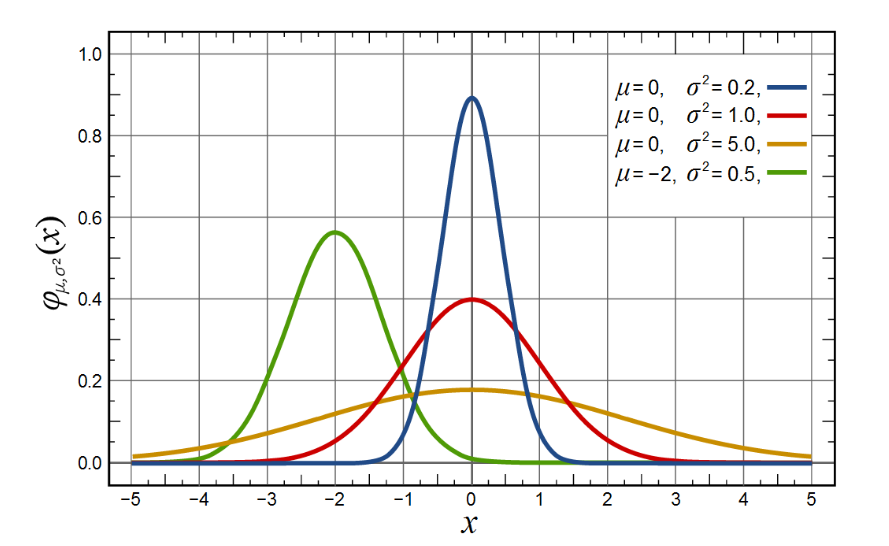
\includegraphics[height=200pt, keepaspectratio = true]{images/gauss}   
\end{figure}
\end{frame}


\begin{frame}\frametitle{Метод максимума правдоподобия}
Метод максимума правдоподобия (ММП):\\
$$L(\varepsilon_1, \dots, \varepsilon_l | w) = \prod\limits_{i=1}^l p(\varepsilon_i) = \prod\limits_{i=1}^l \frac{1}{\sigma_i \sqrt{2\pi}} \exp (-\frac{\varepsilon_i^2}{2\sigma_i^2}  ) \rightarrow \max\limits_{w}$$\\
$$- \ln L(\varepsilon_1, \dots, \varepsilon_l| w) = const(w) + \frac{1}{2} \sum\limits_{i=1}^l \frac{(f(x_i, w) - y_i)^2}{\sigma_i^2}  \rightarrow \min\limits_{w}$$\\
\end{frame}

\begin{frame}\frametitle{Метод максимума правдоподобия}
Метод максимума правдоподобия (ММП):\\
$$- \ln L(\varepsilon_1, \dots, \varepsilon_l| w) = const(w) + \frac{1}{2} \sum\limits_{i=1}^l \frac{(f(x_i, w) - y_i)^2}{\sigma_i^2}  \rightarrow \min\limits_{w}$$\\
\vspace{2mm}
Метод наименьших квадратов: $$Q(w,X^l) = \sum\limits_{i=1}^l \alpha_i (f (x_i, w) - y_i)^2 \rightarrow \min\limits_{w}$$\\
\vspace{5mm}
\textbf{Удивительный факт}: Постановки МНК и ММП, совпадают, причём веса объектов
обратно пропорциональны дисперсии шума, $\alpha_i = \sigma_i^{-2}$
\end{frame}

\begin{frame}\frametitle{Многомерная линейная регрессия}
$f_1(x), \dots, f_n(x)$ -- числовые признаки\\
Модель многомерной линейной регрессии:\\
$$f (x, w) = \sum\limits_{i=1}^l w_j f_j(x), \hspace{5mm} w \in \mathbb{R}$$\\
\vspace{5mm}
Функционал квадрата ошибки:\\
$$Q(w,X^l) = \sum\limits_{i=1}^l (f (x_i, w) - y_i)^2  \rightarrow \min\limits_{w}$$\\

\end{frame}

\begin{frame}\frametitle{Матричное представление}
$$F_{l \times n} = \begin{pmatrix}
  f_1(x_1) & \dots & f_n(x_1) \\
  \dots & \dots & \dots\\
  f_1(x_l) & \dots & f_n(x_l)
 \end{pmatrix} \hspace{1mm} y_{l \times 1} = \begin{pmatrix}
  y_1 \\
  \dots\\
  y_l
 \end{pmatrix} \hspace{1mm} w_{n \times 1} = \begin{pmatrix}
  w_1 \\
  \dots\\
  w_n
 \end{pmatrix}$$ \\
\vspace{5mm}
Функционал квадрата ошибки:\\
$$Q(w,X^l) = \sum\limits_{i=1}^l (f (x_i, w) - y_i)^2  = \Vert Fw - y \Vert^2 \rightarrow \min\limits_{w}$$\\

\end{frame}

\begin{frame}\frametitle{Нормальная система уравнений}
Необходимое условие минимума:\\
$$\frac{\partial Q(w)}{\partial w}  = 2 F^T(F w - y) = 0$$\\
Откуда следует нормальная система задачи МНК:\\
$$F^TFw = F^Ty$$\\
$F^TF$ -- ковариационная матрица признаков $f_1, \dots, f_n$\\
\end{frame}

\begin{frame}\frametitle{Нормальная система уравнений}
Нормальная система задачи МНК:
$$F^TFw = F^Ty$$\\
Решение системы:\\
$$w^* = (F^TF)^{-1}F^Ty = F^+y$$\\
$F^+$ -- псевдообратная матрица\\
\vspace{5mm}
Значение функционала: $Q(w^*) = \Vert P_F y - y \Vert^2$,\\
где $P_F = FF^+ = F(F^TF)^{-1}F^T$ -- проекционная матрица
\end{frame}

\begin{frame}\frametitle{Геометрический смысл}
\begin{figure}[htbp]
  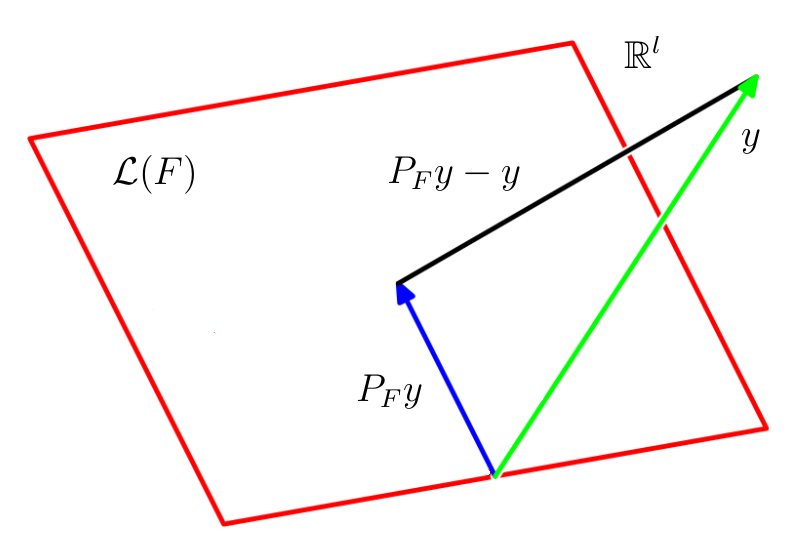
\includegraphics[height=200pt, keepaspectratio = true]{images/geometry}   
\end{figure}
\end{frame}

\begin{frame}\frametitle{Сингулярное разложение}
Произвольная $l \times n$-матрица представима в виде сингулярного разложения:\\
$$F = VDU^T$$\\
Основные свойства сингулярного разложения:\\
\begin{enumerate}[--]
\item $V_{l \times n} = (v_1, \dots, v_n)$ ортогональна, $V^TV = I_n$, \\столбцы $v_j$ - собственные векторы матрицы $FF^T$
\item $U_{n \times n} = (u_1, \dots, u_n)$ ортогональна, $U^TU = I_n$, \\столбцы $u_j$ - собственные векторы матрицы $F^TF$
\item $D$ диагональна, $D_{n \times n} = \operatorname{diag} (\sqrt{\lambda_1}, \dots, \sqrt{\lambda_n})$, \\$\lambda_j > 0$ - собственные значения матриц $F^TF$ и $FF^T$
\end{enumerate}
\end{frame}

\begin{frame}\frametitle{Решение МНК через сингулярное разложение}
Псевдообратная $F^+$, вектор МНК-решения $w^*$,
МНК-аппроксимация целевого вектора $Fw^*$\\
$F^+ = (UDV^TVDU^T)UDV^T = UD^{-1}V^T = \sum\limits_{j=1}^n \frac{1}{\sqrt{\lambda_j}}  u_j v_j^T$\\
$ w^* = F^+y = UD^{-1}V^Ty = \sum\limits_{j=1}^n \frac{1}{\sqrt{\lambda_j}}  u_j (v_j^Ty)$\\
$F w^* = P_F y = (VDU^T)UD^{-1}V^Ty = VV^Ty = \sum\limits_{j=1}^n v_j (v_j^Ty)$\\
$\Vert w^* \Vert^2  = \Vert D^{-1}V^Ty \Vert^2 = \sum\limits_{j=1}^n \frac{1}{\lambda_j} (v_j^Ty)^2$
\end{frame}

\begin{frame}\frametitle{Проблема мультиколлинеарности}
Если $\exists \gamma \in \mathbb{R}^n: F\gamma \approx 0$, то некоторые $\lambda_j$ близки к нулю.\\
Число обусловленности $n \times n$-матрицы $F^TF = A$:
$$\mu(A) = \Vert A \Vert \Vert A^{-1} \Vert = \frac{\max\limits_{u: \Vert u \Vert = 1} \Vert A u \Vert}{\min\limits_{u: \Vert u \Vert = 1} \Vert A u \Vert} = \frac{\lambda_{max}}{\lambda_{min}}$$\\
При умножении обратной матрицы на вектор, $z = A^{-1}u$, относительная погрешность усиливается в $\mu(A)$ раз:\\
$$\frac{\Vert \delta z \Vert}{\Vert z \Vert } \leq \mu(A) \frac{\Vert \delta u \Vert}{\Vert u \Vert }$$
\end{frame}

\begin{frame}\frametitle{Проблема мультиколлинеарности}
Если матрица $F^TF$ плохо обусловлена, то: 
\begin{enumerate}[--]
\item решение становится неустойчивым и неинтерпретируемым, $\Vert w^* \Vert $ велико
\item на обучении $Q(w^*, X^l) = \Vert Fw^* -y \Vert$ -- мало   
\item на контроле $Q(w^*, X^k) = \Vert F'w^* -y' \Vert$ -- велико
\end{enumerate}
\textbf{Вопрос:} Как бороться с этой проблемой?
\end{frame}

\begin{frame}\frametitle{Проблема мультиколлинеарности}
Стратегии устранения мультиколлинеарности и переобучения:
\begin{enumerate}[--]
\item Отбор признаков: $f_1, \dots, f_n \rightarrow f_{j_1}, \dots, f_{j_m}, \hspace{3mm} m << n$
\item Преобразование признаков: $f_1, \dots, f_n \rightarrow g_1, \dots, g_m,\hspace{3mm}  m << n$
\item Регуляризация: $\Vert w \Vert \rightarrow \min$
\end{enumerate}
\end{frame}


\begin{frame}\frametitle{Гребневая регрессия}
Штраф за увеличение нормы вектора весов $\Vert w \Vert$\\
$$Q_{\tau} (w) = \Vert F w - y \Vert^2 + \frac{1}{\sigma} \Vert w \Vert^2$$\\
где $\tau = \frac{1}{\sigma}$ -- неотрицательный параметр регуляризации.\\
%Вероятностная интерпретация: \\
%Априорное распределение вектора $w$ -- гауссовское с ковариационной матрицей $\sigma I_n$.\\
\vspace{5mm}
Модифицированное МНК-решение ($\tau I_n$ — «гребень»)\\
$$w^*_{\tau} = (F^TF + \tau I_n)^{-1}F^Ty$$\\

\textbf{Вопрос:} Можно ли подбирать $\tau$ не вычисляя каждый раз обратную матрицу?
\end{frame}

\begin{frame}\frametitle{Преимущество сингулярного разложения}
Модифицированное МНК-решение ($\tau I_n$ — «гребень»)\\
$$w^*_{\tau} = (F^TF + \tau I_n)^{-1}F^Ty$$\\
Преимущество сингулярного разложения:\\
можно подбирать параметр $\tau$ , вычислив сингулярное разложение только один раз.
\end{frame}

\begin{frame}\frametitle{Сингулярное разложение}
$$w_{\tau}^*= U(D^2 + \tau I_n)^{-1}DV^Ty = \sum\limits_{j=1}^n \frac{\sqrt{\lambda_j}}{\lambda_j + \tau} u_j(v_j^Ty)$$\\
$$Fw_{\tau}^* = VDU^Tw_{\tau}^* = V \operatorname{diag} \left(\frac{\lambda_j}{\lambda_j + \tau}\right) V^Ty = \sum\limits_{j=1}^n \frac{\lambda_j}{\lambda_j + \tau} v_j (v_j^Ty)$$\\
$$\Vert w_{\tau}^* \Vert^2 = \Vert (D^2 + \tau I_n)^{-1} DV^T y \Vert^2 = \sum\limits_{j=1}^n \frac{\lambda_j}{(\lambda_j + \tau)^2} (v^T_j y)^2$$\\
$F w_{\tau}^* \neq Fw^*$ -- зато решение становится более устойчивым
\end{frame}

\begin{frame}\frametitle{Выбор параметра регуляризации $\tau$}
Контрольная выборка: $X^k = (x'_i, y'_i)_{i=1}^k$\\
%Вычисление функционала $Q$ на контрольных данных $T$ раз потребует $O(kn^2 + knT)$ операций:\\
$$Q(w_{\tau}^*,X^k) = \Vert F' w_{\tau}^* - y' \Vert^2 = \Vert F'U \operatorname{diag} \left(\frac{\lambda_j}{\lambda_j + \tau}\right) V^T y -y' \Vert^2$$\\
Зависимость $Q(\tau)$ обычно имеет характерный минимум.
\end{frame}

\begin{frame}\frametitle{Сокращение «эффективной размерности»}
Сокращение весов:\\
$$\Vert w_{\tau}^* \Vert^2 = \sum\limits_{j=1}^n \frac{\lambda_j}{(\lambda_j + \tau)^2} (v^T_j y)^2 < \Vert w^* \Vert^2  = \sum\limits_{j=1}^n \frac{1}{\lambda_j} (v_j^Ty)^2$$\\
Роль размерности играет след проекционной матрицы:\\
$$tr F(F^TF)^{-1}F^T = tr(F^TF)^{-1}F^TF = tr I_n = n$$\\
При использовании регуляризации:\\
$$tr F(F^TF + \tau I_n)^{-1}F^T = tr \hspace{1mm}  \operatorname{diag} \left(\frac{\lambda_j}{\lambda_j + \tau}\right)= \sum\limits_{j=1}^n \frac{\lambda_j}{\lambda_j + \tau } < n $$
\end{frame}

\begin{frame}\frametitle{LASSO}
LASSO -- Least Absolute Shrinkage and Selection Operator\\
$$
\begin{cases} Q(w,X^l) = \Vert Fw - y \Vert^2 \rightarrow \min\limits_{w} \\
\sum_{j=1}^n \vert w_j \vert \leq \kappa
\end{cases}
$$\\
После замены переменных:\\
$$
\begin{cases} w_j = w_j^+ - w_j^-\\
\vert w_j \vert = w_j^+ + w_j^-, \hspace{5mm} w_j^+, w_j^- \geq 0\\

\end{cases}
$$\\
ограничения принимают канонический вид:\\
$$\sum\limits_{j=1}^n w_j^+ + w_j^- \leq \kappa$$\\
Чем меньше $\kappa$, тем больше $j$ таких, что $w_j^+ = w_j^- = 0$\\
%не гауссовское распределение, а лапласовское
\end{frame}

\begin{frame}\frametitle{Негладкие регуляризаторы}
Elastic Net:\\
$$\frac{1}{2} \Vert Fw - y \Vert^2 + \mu \sum\limits_{j=1}^n \vert w_j \vert + \frac{\tau}{2} \sum\limits_{j=1}^n w_j^2 \rightarrow \min\limits_{w}$$\\
Support Features Machine:\\
$$\frac{1}{2} \Vert Fw - y \Vert^2 + \tau \sum\limits_{j=1}^n R_{\mu}(w_j) \rightarrow \min\limits_{w}$$\\
$$ R_{\mu}(w_j) = \begin{cases} 2 \mu \vert w_j \vert, \hspace{2mm} \vert w_j \vert \leq \mu\\
\mu^2 + w_j^2, \hspace{2mm} \vert w_j \vert \geq \mu
\end{cases}$$\\
%Применение этих методов требует выбора траектории регуляризации в пространстве $(\mu, \tau )$
\end{frame}

\begin{frame}\frametitle{Метод главных компонент}
$f_1(x), \dots, f_n(x)$ -- исходные числовые признаки\\
$g_1(x), \dots, g_m(x)$ -- новые числовые признаки, $m \times n$\\
\vspace{5mm}
\textbf{Вопрос:} Как сформулировать требование к новым признакам?
\end{frame}


\begin{frame}\frametitle{Метод главных компонент}
$f_1(x), \dots, f_n(x)$ -- исходные числовые признаки\\
$g_1(x), \dots, g_m(x)$ -- новые числовые признаки, $m \times n$\\
Требование: старые признаки должны линейно
восстанавливаться по новым:\\
$$\hat{f}_j(x) = \sum\limits_{s=1}^m g_s(x) u_{js} , \hspace{2mm} j = 1,\dots , n, \hspace{2mm} \forall x \in X$$\\
как можно точнее на обучающей выборке $x_1, \dots, x_l$:\\
$$\sum\limits_{i=1}^l \sum\limits_{j=1}^n (\hat{f}_j(x_i) - f_j(x_i))^2 \rightarrow \min\limits_{g_s(x_i), u_{js}}$$
\end{frame}

\begin{frame}\frametitle{Матричные обозначения}
$$F_{l \times n} = \begin{pmatrix}
  f_1(x_1) & \dots & f_n(x_1) \\
  \dots & \dots & \dots\\
  f_1(x_l) & \dots & f_n(x_l)
 \end{pmatrix} \hspace{1mm} G_{l \times m} = \begin{pmatrix}
  g_1(x_1) & \dots & g_m(x_1) \\
  \dots & \dots & \dots\\
  g_1(x_l) & \dots & g_m(x_l)
 \end{pmatrix}$$\\
 $$U_{n \times m} = \begin{pmatrix}
  u_{11} & \dots & u_{1m} \\
  \dots & \dots & \dots\\
  u_{n1} & \dots & u_{nm}
 \end{pmatrix}$$
$U$ -- линейное преобразование новых признаков в старые\\
$$\hat{F} = GU^T \approx F$$\\
Найти: новые признаки $G$ и преобразование $U$:\\
$$\sum\limits_{i=1}^l \sum\limits_{j=1}^n (\hat{f}_j(x_i) - f_j(x_i))^2 = \Vert GU^T - F \Vert^2 \rightarrow \min\limits_{G, U}$$
\end{frame}

\begin{frame}\frametitle{Основная теорема}
Если $m < \rank F$, то минимум $\Vert GU^T - F \Vert^2$ достигается, когда столбцы $U$ - это с.в. матрицы $F^TF$, соответствующие $m$ максимальным с.з. $\lambda_1,\dots, \lambda_m$, а матрица $G = FU$.\\
\vspace{5mm}
При этом:\\
\begin{enumerate}[--]
\item матрица $U$ ортонормирована: $U^TU = I_m$
\item матрица $G$ ортогональна: $G^TG = \Lambda = \operatorname{diag}(\lambda_1, \dots, \lambda_m)$
\item $U\Lambda = F^TFU$,  $G\Lambda = FF^TG$
\item $\Vert GU^T - F \Vert^2 = \Vert F \Vert^2 - tr \Lambda = \sum\limits_{j=m+1}^n \lambda_j$
\end{enumerate}

\end{frame}

\begin{frame}\frametitle{Связь с сингулярным разложением}
Если взять $m = n$, то:\\
\begin{enumerate}[--]
\item $\Vert GU^T - F \Vert^2 = 0$
\item представление $\hat{F} = GU^T = F$ точное и совпадает с сингулярным разложением при $G = V \sqrt{\Lambda}$
$$F = GU^T = V\sqrt{\Lambda}U^T, \hspace{2mm} U^TU = I_m, \hspace{2mm} V^TV = I_m$$
\item линейное преобразование $U$ работает в обе стороны:\\
$$F= GU^T, \hspace{4mm} G=FU$$
Преобразование $U$ называется декоррелирующим
\end{enumerate}
\end{frame}

\begin{frame}\frametitle{Эффективная размерность выборки}
Упорядочим с.з. $F^TF$ по убыванию: $\lambda_1 > \dots > \lambda_n > 0$\\
Эффективная размерность выборки -- это наименьшее целое $m$, при котором\\
$$E_m = \frac{\Vert GU^T - F \Vert^2}{\Vert F \Vert^2} = \frac{\lambda_{m+1} + \dots + \lambda_{n}}{\lambda_1 + \dots + \lambda_n} \leq \varepsilon$$\\
Критерий «крутого склона»: находим $m: E_m-1 >> E_m$:
\begin{figure}[htbp]
  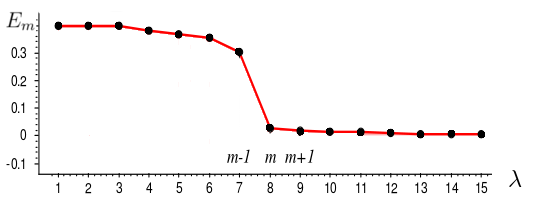
\includegraphics[height=100pt, keepaspectratio = true]{images/edge}   
\end{figure}
\end{frame}

\begin{frame}\frametitle{Решение задачи НК в новых признаках}
Заменим $F$ на её приближение $GU^T$:\\
$$\Vert GU^Tw -y \Vert^2 = \Vert G\hat{w} -y \Vert^2 \rightarrow \min\limits_{\hat{w}}$$\\
Связь нового и старого вектора коэффициентов:\\
$$w = U\hat{w}, \hspace{5mm} \hat{w} = U^T w$$\\
Решение задачи наименьших квадратов относительно $\hat{w}$ (единственное отличие -- $m$ слагаемых вместо $n$):\\
$$\hat{w}^* = D^{-1}V^Ty = \sum\limits_{j=1}^m \frac{1}{\sqrt{\lambda_j}} u_j (v_j^Ty)$$\\
$$G\hat{w}^* = VV^Ty = \sum\limits_{j=1}^m v_j (v_j^Ty)$$
\end{frame}

\begin{frame}\frametitle{Нелинейная регрессия}
\textbf{Вопрос:} Что изменится, если модель регрессии не линейна?\\
\vspace{5mm}
$$f(x, w), \hspace{5mm} w \in \mathbb{R}^p$$
\end{frame}


\begin{frame}\frametitle{Метод Ньютона-Рафсена}
Начальное приближение $w^{(0)} = (w_1^{(0)}, \dots, w_p^{(0)})$\\
Итерационный процесс: $w^{(t+1)} = w^{(t)} - h_t (Q''(w^{(t)}))^{-1}Q'(w^{(t)})$\\
\vspace{5mm}
$Q'(w^{(t)})$ -- градиент функционала $Q$ в точке $w^{(t)}$\\
$Q''(w^{(t)})$ -- гессиан функционала $Q$ в точке $w^{(t)}$\\
$h_t$ -- величина шага
\end{frame}

\begin{frame}\frametitle{Метод Ньютона-Рафсена}
$\frac{\partial Q(w)}{\partial w_j} = 2 \sum\limits_{i=1}^l (f(x_i, w) - y_i ) \frac{\partial(f(x_i, w))}{\partial w_j}$\\
$\frac{\partial^2 Q(w)}{\partial w_j \partial w_k} = 2 \sum\limits_{i=1}^l \frac{\partial(f(x_i, w))}{\partial w_j} \frac{\partial(f(x_i, w))}{\partial w_k} - 2 \sum\limits_{i=1}^l (f(x_i, w) - y_i ) \frac{\partial^2 (f(x_i, w))}{\partial w_j \partial w_k}$\\
\vspace{5mm}
\textbf{Вопрос:} Какая часть самая тяжелая?
\end{frame}

\begin{frame}\frametitle{Метод Ньютона-Рафсена}
$\frac{\partial Q(w)}{\partial w_j} = 2 \sum\limits_{i=1}^l (f(x_i, w) - y_i ) \frac{\partial(f(x_i, w))}{\partial w_j}$\\
$\frac{\partial^2 Q(w)}{\partial w_j \partial w_k} = 2 \sum\limits_{i=1}^l \frac{\partial(f(x_i, w))}{\partial w_j} \frac{\partial(f(x_i, w))}{\partial w_k} - 2 \sum\limits_{i=1}^l (f(x_i, w) - y_i ) \frac{\partial^2 (f(x_i, w))}{\partial w_j \partial w_k}$\\
\vspace{5mm}
Линеаризация $f(x_i, w)$ в окрестности текущего $w^{(t)}$:\\
$f(x_i, w) = f(x_i, w^{(t)}) + \sum\limits_{j=1}^p \frac{\partial(f(x_i, w))}{\partial w_j} (w_j - w_j^{(t)}) + o(w_j -w_j^{(t)})$\\
$\Rightarrow$ второе слагаемое в гессиане обнулилось
\end{frame}

\begin{frame}\frametitle{Метод Ньютона-Рафсена}
\begin{figure}[htbp]
  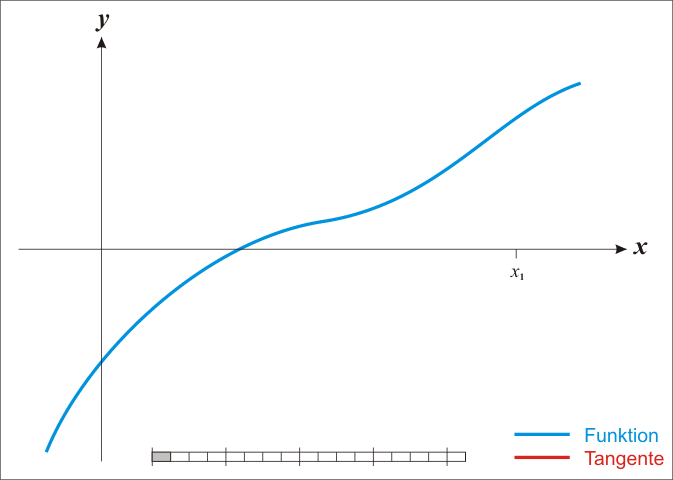
\includegraphics[height=150pt, keepaspectratio = true]{images/newton-1}   
\end{figure}
\end{frame}

\begin{frame}\frametitle{Метод Ньютона-Рафсена}
\begin{figure}[htbp]
  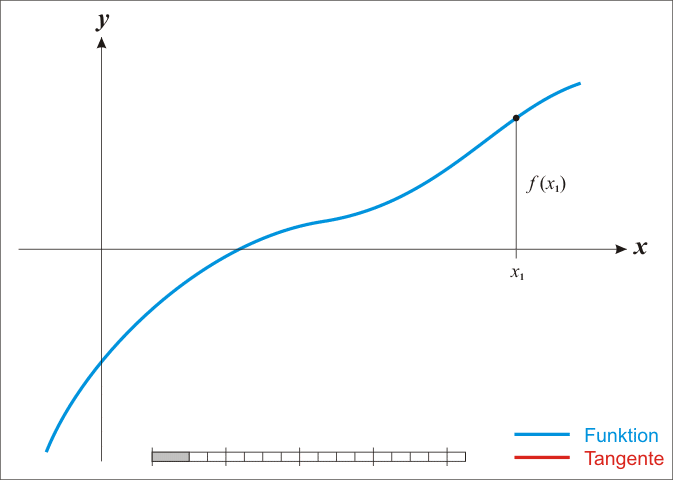
\includegraphics[height=150pt, keepaspectratio = true]{images/newton-2}   
\end{figure}
\end{frame}

\begin{frame}\frametitle{Метод Ньютона-Рафсена}
\begin{figure}[htbp]
  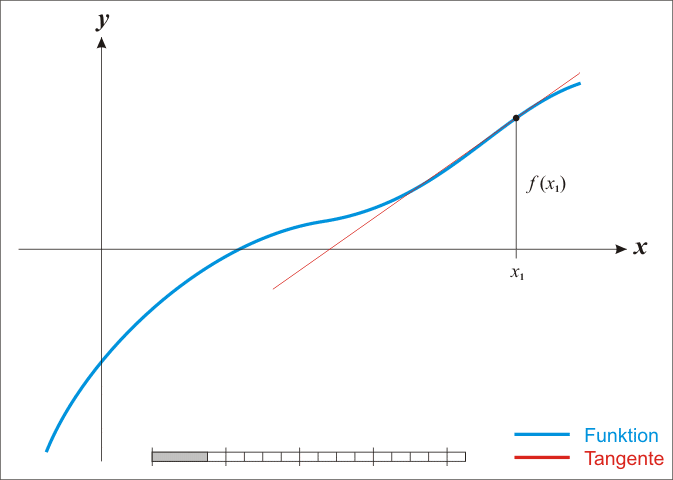
\includegraphics[height=150pt, keepaspectratio = true]{images/newton-3}   
\end{figure}
\end{frame}
\begin{frame}\frametitle{Метод Ньютона-Рафсена}
\begin{figure}[htbp]
  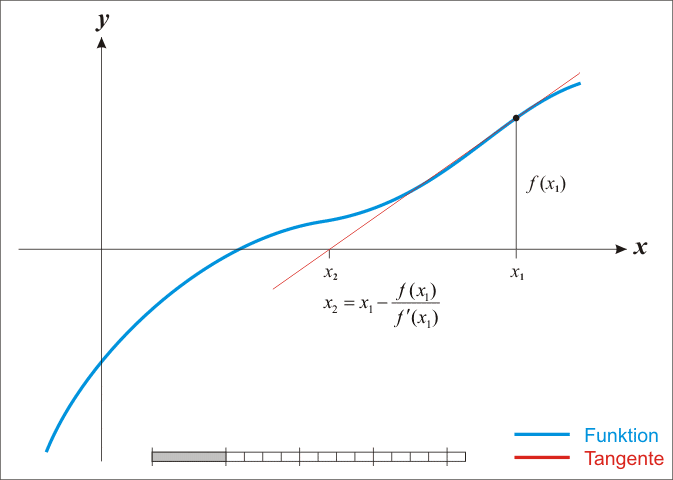
\includegraphics[height=150pt, keepaspectratio = true]{images/newton-4}   
\end{figure}
\end{frame}
\begin{frame}\frametitle{Метод Ньютона-Рафсена}
\begin{figure}[htbp]
  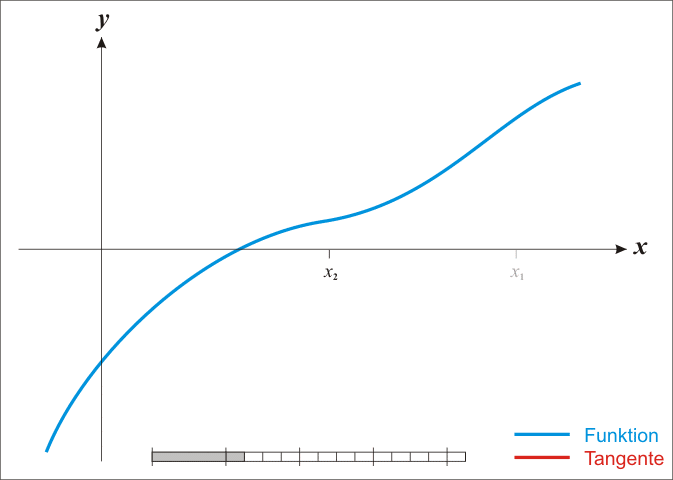
\includegraphics[height=150pt, keepaspectratio = true]{images/newton-5}   
\end{figure}
\end{frame}
\begin{frame}\frametitle{Метод Ньютона-Рафсена}
\begin{figure}[htbp]
  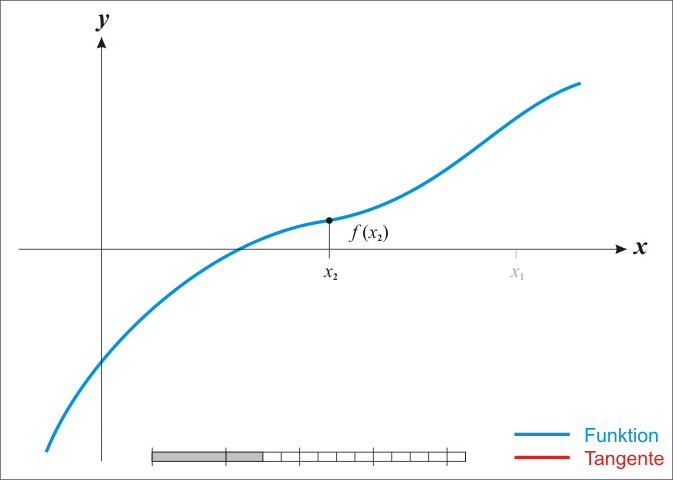
\includegraphics[height=150pt, keepaspectratio = true]{images/newton-6}   
\end{figure}
\end{frame}
\begin{frame}\frametitle{Метод Ньютона-Рафсена}
\begin{figure}[htbp]
  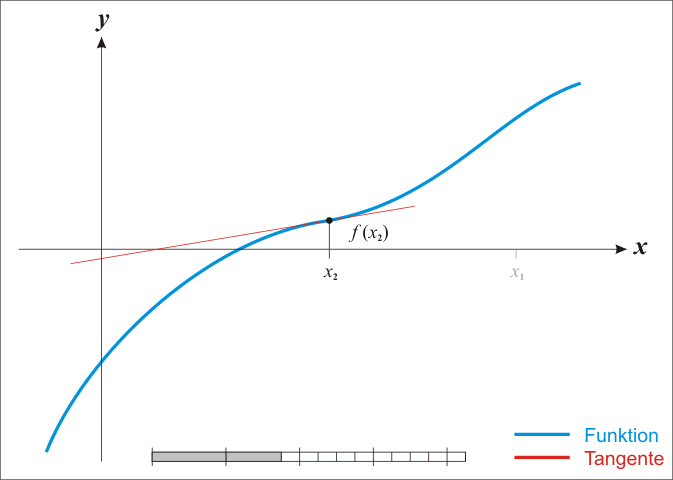
\includegraphics[height=150pt, keepaspectratio = true]{images/newton-7}   
\end{figure}
\end{frame}
\begin{frame}\frametitle{Метод Ньютона-Рафсена}
\begin{figure}[htbp]
  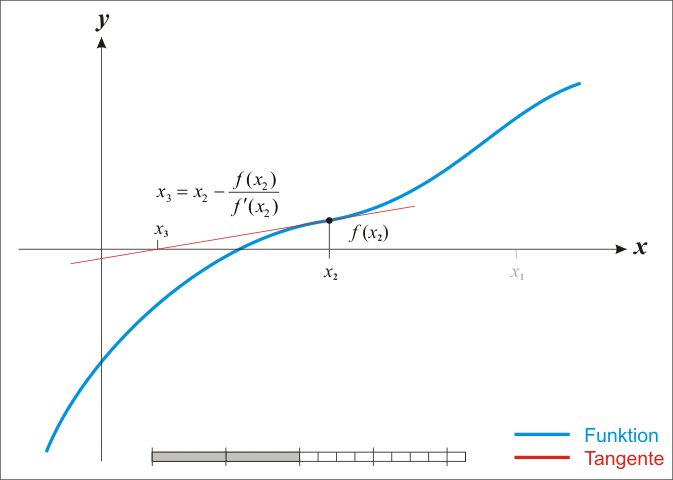
\includegraphics[height=150pt, keepaspectratio = true]{images/newton-8}   
\end{figure}
\end{frame}
\begin{frame}\frametitle{Метод Ньютона-Рафсена}
\begin{figure}[htbp]
  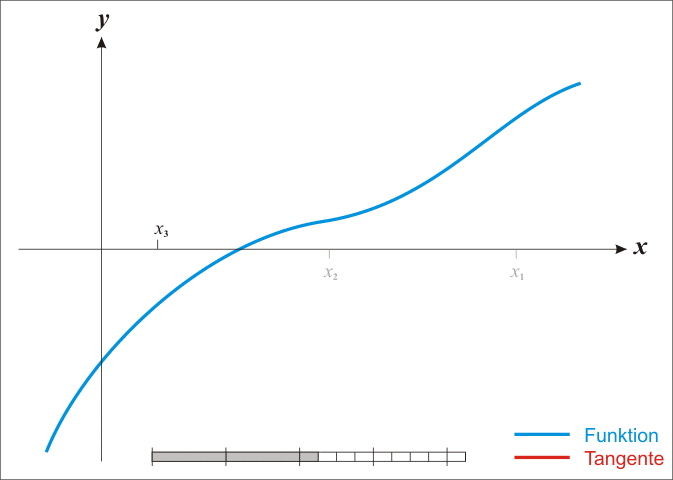
\includegraphics[height=150pt, keepaspectratio = true]{images/newton-9}   
\end{figure}
\end{frame}
\begin{frame}\frametitle{Метод Ньютона-Рафсена}
\begin{figure}[htbp]
  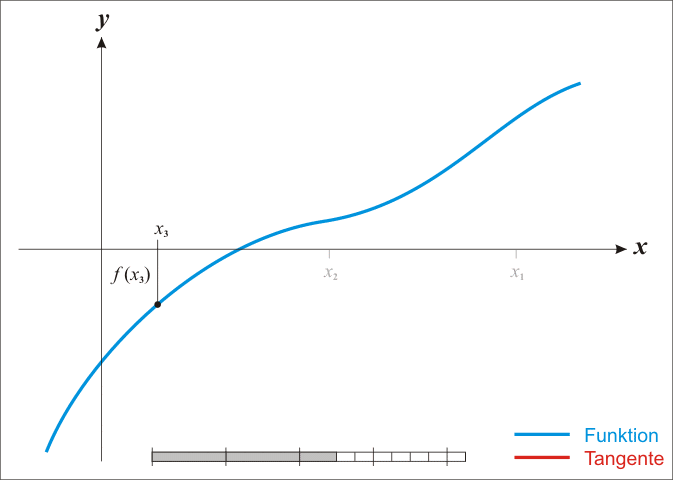
\includegraphics[height=150pt, keepaspectratio = true]{images/newton-10}   
\end{figure}
\end{frame}
\begin{frame}\frametitle{Метод Ньютона-Рафсена}
\begin{figure}[htbp]
  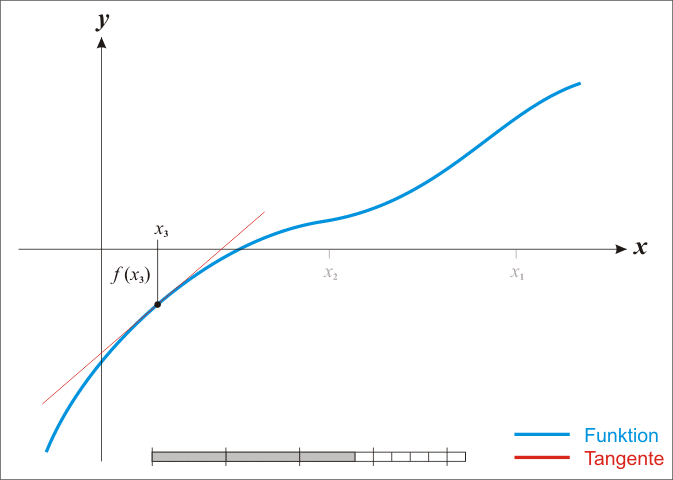
\includegraphics[height=150pt, keepaspectratio = true]{images/newton-11}   
\end{figure}
\end{frame}
\begin{frame}\frametitle{Метод Ньютона-Рафсена}
\begin{figure}[htbp]
  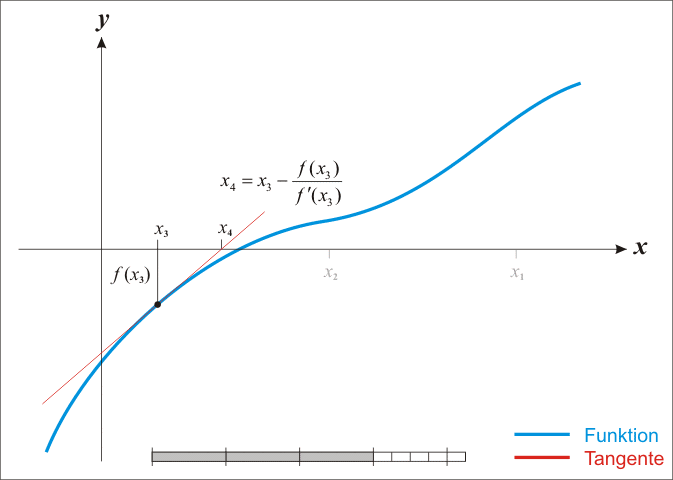
\includegraphics[height=150pt, keepaspectratio = true]{images/newton-12}   
\end{figure}
\end{frame}
\begin{frame}\frametitle{Метод Ньютона-Рафсена}
\begin{figure}[htbp]
  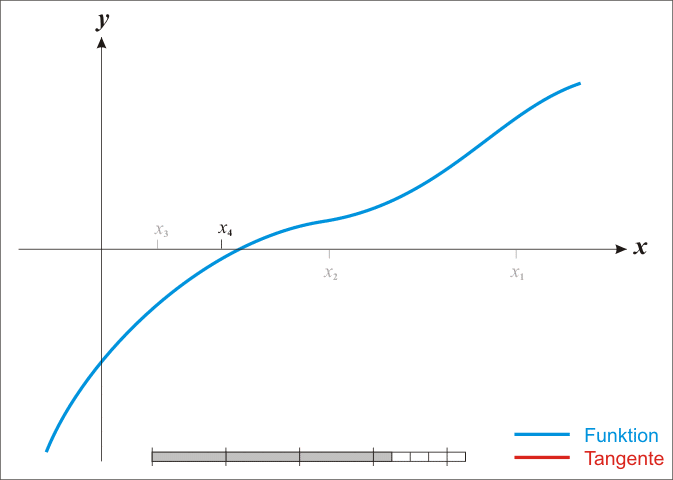
\includegraphics[height=150pt, keepaspectratio = true]{images/newton-13}   
\end{figure}
\end{frame}
\begin{frame}\frametitle{Метод Ньютона-Рафсена}
\begin{figure}[htbp]
  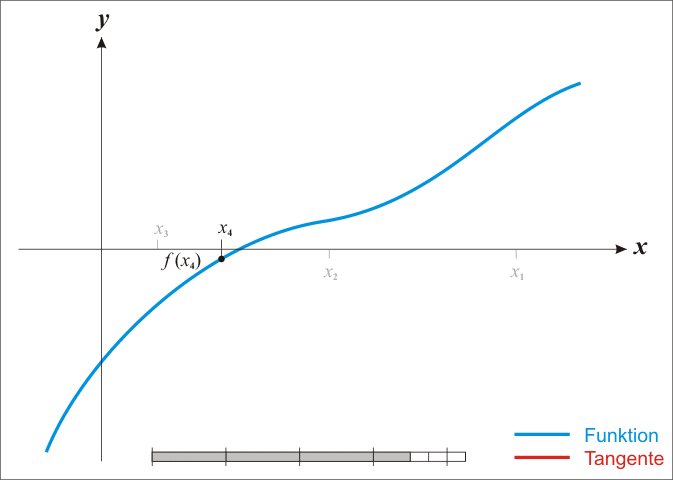
\includegraphics[height=150pt, keepaspectratio = true]{images/newton-14}   
\end{figure}
\end{frame}
\begin{frame}\frametitle{Метод Ньютона-Рафсена}
\begin{figure}[htbp]
  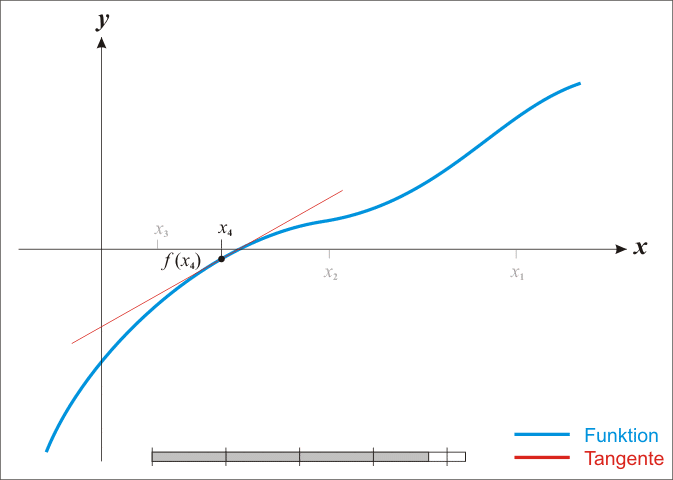
\includegraphics[height=150pt, keepaspectratio = true]{images/newton-15}   
\end{figure}
\end{frame}
\begin{frame}\frametitle{Метод Ньютона-Рафсена}
\begin{figure}[htbp]
  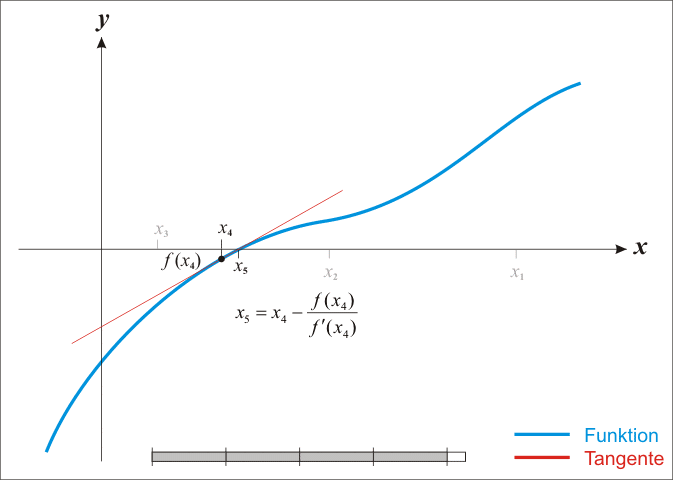
\includegraphics[height=150pt, keepaspectratio = true]{images/newton-16}   
\end{figure}
\end{frame}
\begin{frame}\frametitle{Метод Ньютона-Рафсена}
\begin{figure}[htbp]
  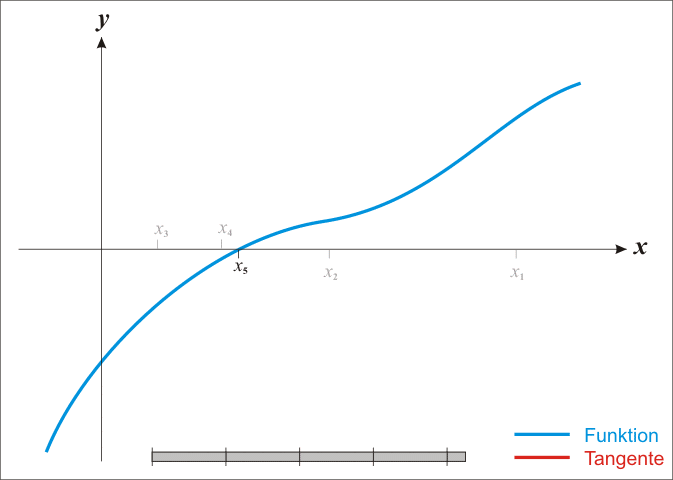
\includegraphics[height=150pt, keepaspectratio = true]{images/newton-17}   
\end{figure}
\end{frame}

\begin{frame}\frametitle{Матричные обозначения}
$F_t = \left(\frac{\partial(f(x_i, w))}{\partial w_j^{(t)}}\right)_{l \times p}$ -- матрица первых производных\\
$f_t = \left( f(x_i, w^{(t)}) \right)_{l \times 1}$ -- вектор значений $f$\\
\vspace{5mm}
Формула $t$-й итерации метода Ньютона–Гаусса:\\
$$w^{(t+1)} = w^{(t)} - h_t \underbrace{\left( F^T_tF_t \right)^{-1} F_t^T(f_t -y)}_{\beta}$$\\
где $\beta$ -- решение многомерной линейной регрессии\\
$$\Vert F_t\beta - (f_t-y) \Vert^2 \rightarrow \min_{\beta}$$ 
\end{frame}

%\begin{frame}\frametitle{ROC кривая}
%\end{frame}


\begin{frame}\frametitle{На следующей лекции}
\begin{itemize}
\item[--] Нейронные сети
\end{itemize}
\end{frame}
\end{document}
